\subsection{Ethereum}
        Ethereum\cite{ethereum} (figure \ref{fig:ethereum_logo}) is an open-source, public, blockchain-based distributed ledger featuring smart contract functionality. It enables developers to build blockchain applications with business logic that execute in a trustless environment, while leveraging the high availability of the Ethereum network. 
        \begin{figure}[h]
            \centering
            
\includegraphics[width=0.5\textwidth]{ethereum-logo-portrait-purple.png}
            \caption{Ethereum logo}
            \label{fig:ethereum_logo}
        \end{figure}
        The principles behind Ethereum philosophy are\cite{ethereumWhitepaper}:
        \begin{itemize}
            \item \textbf{Simplicity}. The Ethereum protocol should be as simple as possible.
            \item \textbf{Universality}. Ethereum provides an internal Turing-complete scripting language. This language can be used to construct any logic, and any business case.
            \item \textbf{Modularity}. The Ethereum protocol is designed to be as modular as possible, to allow if one was to make a small protocol modification in one place, the application stack would continue to function as normally. 
            \item \textbf{Agility}. The protocol can be modified.
            \item \textbf{Non-discrimination} and \textbf{non-censorship}. The protocol should not restrict any usage.
        \end{itemize}
        
        \subsubsection{Ether}
            \acrfull{eth} is the native cryptocurrency used on the Ethereum network and is used to compensate miners who secure transactions. It is used to pay for gas, a unit of computation used in transactions and other state transitions.
            \acrlong{eth} also has many current use cases, such as a store of value, a medium of exchange, and a unit of account.
            
        \subsubsection{Ethereum Accounts}
            An Ethereum account or simply an "account" is the combination of an Ethereum address and it's private key. An account can hold balance (\acrlong{eth}) and can send transactions. In Ethereum there are 2 types of accounts.
            \begin{itemize}
                \item \textbf{\acrfull{eoa}}. These accounts are a combination of public address and private key. This accounts:
                \begin{itemize}
                    \item Has an \acrlong{eth} balance
                    \item Can send transactions to Smart Contracts
                    \item Can send and receive \acrlong{eth} to/from another account
                    \item Is controlled by private keys
                    \item Has no associated code
                \end{itemize}
                \item \textbf{Contract accounts}: These accounts don't have a corresponding private key. These accounts are generated when a Smart Contract is deployed in the blockchain. They are normally called "contracts" instead of contract accounts. A contract:
                \begin{itemize}
                    \item Has an \acrlong{eth} balance
                    \item They can receive \acrlong{eth} just like \acrshort{eoa}
                    \item Has associated code
                    \item Code execution is triggered by transactions or calls received from other contracts or accounts
                    \item When executed can manipulate its own persistent storage
                \end{itemize}
            \end{itemize}
        
        \subsubsection{Ethereum wallet}
            Wallets are software that are used to store and manage Ethereum accounts. Wallets allow the user to manage multiple accounts, provide functionality to sign transactions, track balances and so on. Wallets can be classified into two types.
            \begin{itemize}
                \item \textbf{Non-deterministic} wallet. These wallets use a random private key and generate a private key from it.
                \item \textbf{Deterministic} wallet. In this wallet, keys are derived from a seed. The seed allows a user to easily back up and restore a wallet without needing any other information, and in some cases allow the creation of public addresses without the knowledge of the private key.
            \end{itemize}
        
        \subsubsection{Ethereum stack}
            Like any software stack, the complete "Ethereum stack"\cite{ethereumStack} will vary from project to project depending on your business goals. However, the typical layers are:
            \paragraph{Ethereum Virtual Machine (EVM)}
                The \acrlong{evm}\cite{evm}, normally known as \acrshort{evm} is a software designed to emulate a machine with certain capabilities that make the Ethereum blockchain possible. We can program instructions for the \acrshort{evm}, using a series of opcodes, which we can then compile and translate into a specific bytecode or language that the \acrshort{evm} can understand and execute.\\
                
                The opcodes perform standard stack operations like \textit{XORAND}, \textit{ADD}, \textit{SUB}, etc. The \acrshort{evm} also implements a number of blockchain-specific stack operations, such as \textit{ADDRESS}, \textit{BALANCE}, \textit{SHA3}, \textit{BLOCKHASH}, etc. More specific information can be found at the official documentation\cite{opcodes}.\\
                
                To make programming easier for the virtual machine, a specialized high-level language called Solidity was created. This programming language is used to create Smart Contracts. Solidity first transforms opcodes and then these to bytecode. This bytecode is finally executed by the \acrshort{evm} to perform the specified operations of a  Smart Contract. All this means that the \acrshort{evm} can function as a real computer, executing from the simplest to the most complex operations.\\
                
                In the following sections we will talk in detail about the Smart Contracts and Solidity.
                
            \paragraph{EVM Characteristics}
                The \acrshort{evm} has a series of unique characteristics\cite{ethereumGavin,ethereumDocu}:
                \begin{itemize}
                    \item It provides a \textbf{high level of security}. As it is a virtual machine limited in the instructions (opcodes) and the way they are executed, \acrshort{evm} is capable of executing unreliable codes without disastrous consequences.
                    \item The \acrshort{evm} is a \textbf{completely decentralized} build. Each node within the Ethereum network runs a copy of the virtual machine and is synchronized with the rest of the nodes that make up the network. This guarantees that the instructions given by the \acrshort{evm} are executed as long as there is at least one active node. This allows access to the system from anywhere in the world, resisting censorship and guaranteeing access to network resources. Furthermore, it does not require the participation of third parties, and resources can't be modified or altered.
                    \item Applications can be executed on the same blockchain network, without affecting other operations.
                    \item \acrshort{evm} is able to follow the "rules" of Smart Contracts.
                    \item The \acrshort{evm} has the ability to execute a series of well-defined opcodes.
                \end{itemize}
                
            \paragraph{How does it work?}
                The figure \ref{fig:blockchain_stack} defines how the \acrshort{evm} works\cite{queEsEvm}.
                \begin{figure}[h]
                    \centering
                    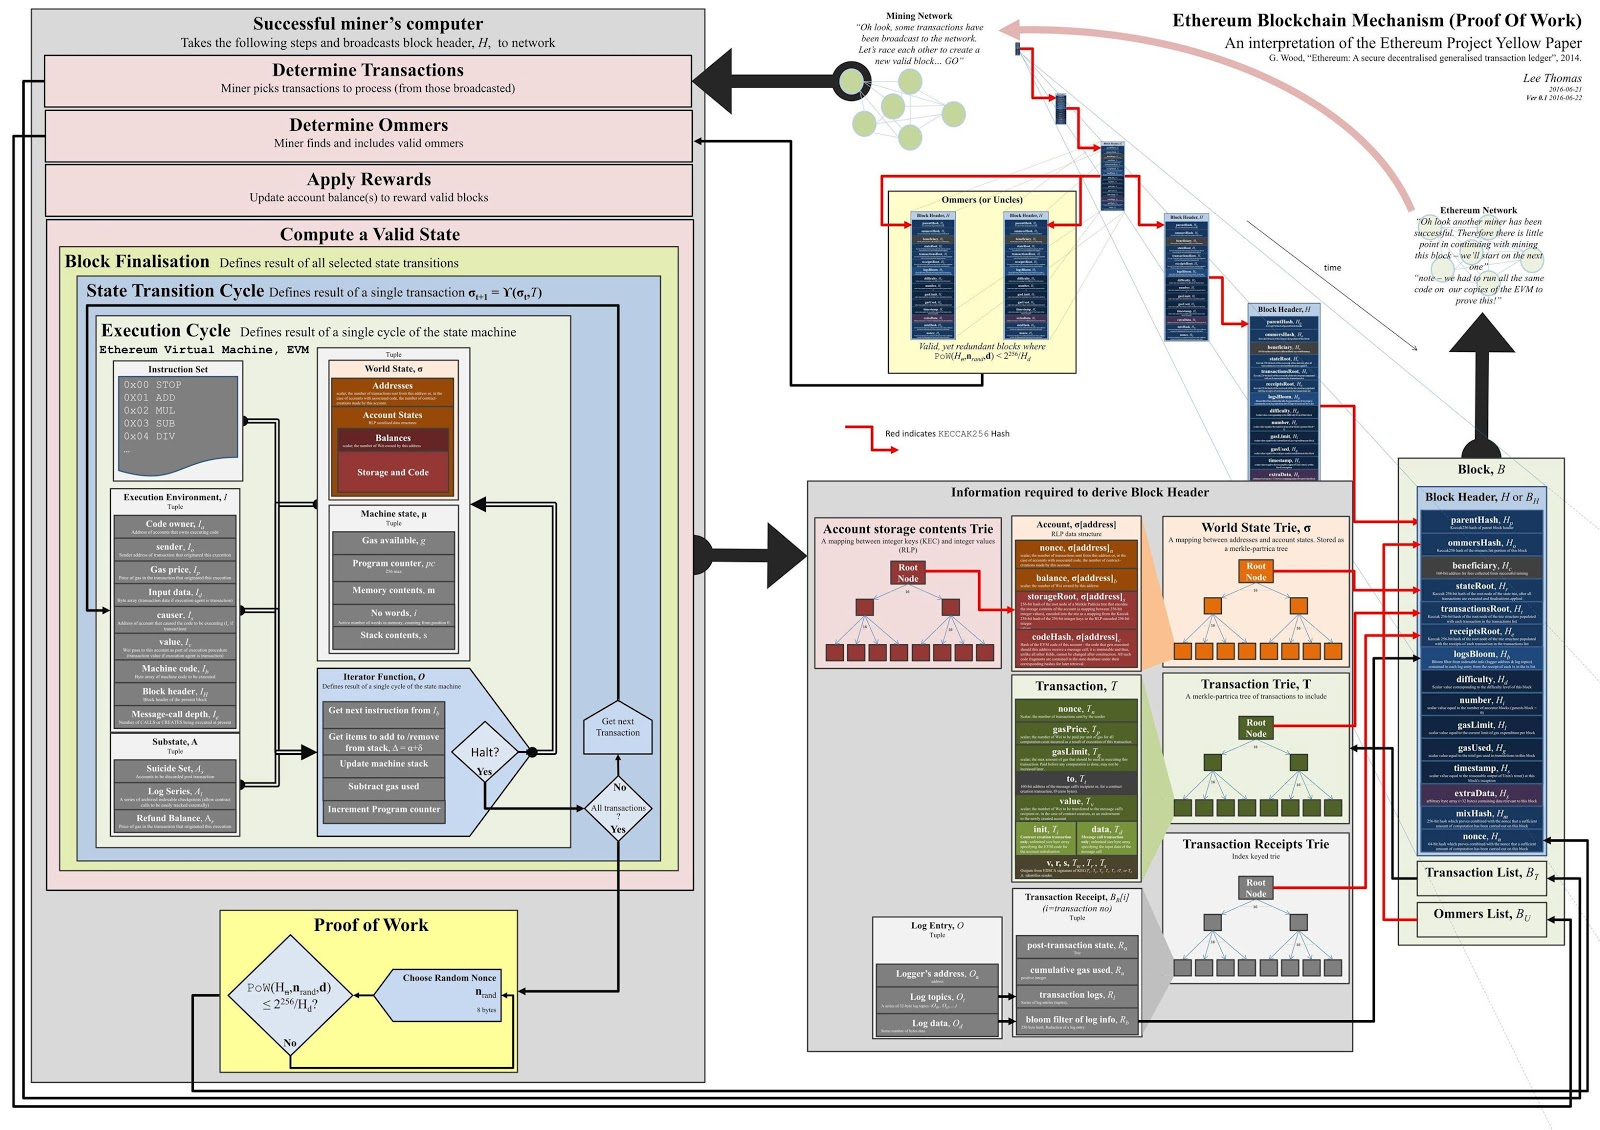
\includegraphics[width=1\textwidth]{evm-stack.jpeg}
                    \caption{\acrshort{evm} stack schema}
                    \label{fig:blockchain_stack}
                \end{figure}

                The Smart Contracts made with Solidity are compiled and converted to opcodes. These opcodes are transformed to bytecode, so it does facilitate the performance of the \acrshort{evm} tasks.\\

                Thus, each transaction and operation that is carried out on the Ethereum blockchain goes through this process, and its execution is carried out by the \acrshort{evm}, which at the end records everything on the Ethereum blockchain, leaving a public record of those operations. 

        \subsubsection{Smart Contracts}
            Sam Richards\cite{smartContracts}, a Software Engineer working on Ethereum defines the Smart Contract as 
            \begin{quote}
                \textit{a snippet of code that runs on the Ethereum blockchain. It's a collection of functions and data that resides at a specific address on the Ethereum blockchain.}

                \textit{Smart contracts are a type of Ethereum account. This means they have a balance and they can send transactions over the network. However they're not controlled by a user, instead they are deployed to the network and run as programmed. User accounts can then interact with a smart contract by submitting transactions that execute a function defined on the smart contract. Smart contracts can define rules, like a regular contract, and automatically enforce them via the code.}
            \end{quote}

        \subsubsection{Solidity}
            \begin{figure}[h]
                \centering
                
\includegraphics[width=0.4\textwidth]{solidity-logo.jpg}
                \caption{Solidity logo}
                \label{fig:solidity_logo}
            \end{figure}
            
            Solidity (figure \ref{fig:solidity_logo}) defines itself as an object-oriented, high-level language for implementing Smart Contracts. Smart Contracts are programs which govern the behaviour of accounts within the Ethereum state.\\
            
            Solidity\cite{solidityGit} was influenced by \textit{C++}, \textit{Python} and \textit{JavaScript} and is designed to target the \acrfull{evm}. Solidity is statically typed, supports inheritance, libraries and complex user-defined types among other features.\\

            Below is an example of a Smart Contract\footnote{Source code from \url{https://github.com/alastria/alastria-identity/blob/master/contracts/identityManager/AlastriaIdentityIssuer.sol}} written in Solidity\footnote{More details about Solidity can be found in the official documentation\cite{solidity}} (listing  \ref{lst:AlastriaIdentityIssuer}).
            
            \lstinputlisting[label={lst:AlastriaIdentityIssuer}, caption=Source code from AlastriaIdentityIssuer.sol, language=Solidity]{examples/alastriaSCs/identityManager/AlastriaIdentityIssuer.sol}

        \subsubsection{Ethereum Nodes}
            A Node refers to a piece of software which is an implementation of Ethereum that verifies all transactions in each block, keeping the network secure and the data accurate. They collectively store the state of the Ethereum blockchain and reach consensus on transactions to mutate the blockchain state.\\
            
            There are three types of nodes.
            \begin{itemize}
                \item \textbf{Full node}. These types of nodes store full blockchain data, participate in block validation, verifies all blocks and states and serves the network and provides data on request. Also, all states can be derived from a full node.
                \item \textbf{Light node}. Stores the header chain and requests everything else. Can verify the validity of the data against the state roots in the block headers and it is useful for low capacity devices, such as embedded devices or mobile phones, which can't afford to store gigabytes of blockchain data.
                \item \textbf{Archive node}. Stores everything kept in the full node and builds an archive of historical states. These nodes can be handy for services like block explorers, wallet vendors, and chain analytics.
            \end{itemize}
            By connecting your application to an Ethereum node via \acrshort{json} \acrshort{rpc}, your application is able to read data from the blockchain as well as broadcast new transactions to the network.

        \subsubsection{Ethereum Client APIs}
            While APIs are not a necessary piece of the stack, they abstract away much of the complexity of interacting directly with Ethereum nodes and Smart contracts.\\
            
            Most of these APIs are open source and maintained by the Ethereum community.

        \subsubsection{End User Applications}
            The final part of the stack is the user-facing applications, primarily web and mobile apps.  They are made for users so they do not need to know the application they're using is built using a blockchain. Also the end user applications are made to hide the complexity from the user.
            
        \subsubsection{Ethereum 2.0 (Eth2)}
            \acrshort{eth2}\cite{eth2} is a long-planned upgrade to the Ethereum network, it will reduce energy consumption, allow the network to process more transactions, and increase security.  Ethereum will become a proof-of-stake blockchain and introduce shard chains. Shard chains are like parallel blockchains that sit within Ethereum and take on a portion of the network's processing work.\\
            
            The phase 1 of Ethereum 2.0 is supposed to happen in 2021. The roadmap can be checked in the official website\cite{eth2Roadmap}.

